\documentclass{llncs}

\usepackage{graphicx}
\usepackage{xcolor}
\usepackage{listings}
\usepackage{booktabs}
\usepackage{float}
\usepackage{tikz}
\usetikzlibrary{shapes.geometric, arrows.meta, positioning, fit, backgrounds}
\usepackage{url}

% --- DEFINIR A LINGUAGEM JSON ---
\lstdefinelanguage{json}{
    basicstyle=\normalfont\ttfamily\scriptsize,
    showstringspaces=false,
    breaklines=true,
    string=[s]{"}{"},
    stringstyle=\color{blue},
    comment=[l]{:},
    commentstyle=\color{black},
}

% --- FLOAT PLACEMENT: evitar paginas so com floats e whitespace ---
% Por defeito o LaTeX recusa-se a por um float grande numa pagina com texto,
% empurrando-o para uma pagina propria (era o caso da Fig. 2). Estes valores
% deixam um float ocupar ate 90% de uma pagina partilhada com texto.
\renewcommand{\topfraction}{0.9}
\renewcommand{\bottomfraction}{0.8}
\renewcommand{\textfraction}{0.07}
\renewcommand{\floatpagefraction}{0.75}
\setcounter{topnumber}{3}
\setcounter{bottomnumber}{2}
\setcounter{totalnumber}{4}
% Separacao entre floats e texto (LNCS usa ~20pt por defeito).
\setlength{\textfloatsep}{8pt plus 2pt minus 4pt}
\setlength{\floatsep}{8pt plus 2pt minus 4pt}
\setlength{\intextsep}{8pt plus 2pt minus 4pt}

% --- COMPRIMIR BIBLIOGRAFIA ---
\let\oldbibliography\thebibliography
\renewcommand{\thebibliography}[1]{%
  \oldbibliography{#1}%
  \setlength{\itemsep}{0pt}%
  \setlength{\parskip}{0pt}%
}



% margem extra para o TeX resolver linhas ligeiramente overfull
\emergencystretch=1.5em

\begin{document}

\title{MARTA: A Decoupled Multi-Agent Architecture for Python Test Generation}


% ICTSS 2026 e DOUBLE-BLIND: sem nomes nem afiliacoes na submissao.
% Preencher com os autores reais so na camera-ready.
\author{Anonymous}
\institute{Anonymous}
\maketitle

\begin{abstract}

Recent Large Language Model (LLM) frameworks for Python test generation use static analysis to construct rich semantic contexts, yet their generation phase typically relies on a single prompt that combines test planning, code synthesis, and assertion design. This coupling often leads to context dilution, invalid assertions, and tests that execute code without verifying behaviour. We present MARTA (Multi-Agent Refinement and Testing Architecture), a Python test generation pipeline that separates abstract test planning from concrete test implementation. A Planner Agent designs logical test scenarios, while an Assertion Agent translates each plan into a complete Pytest file. By introducing test plans as an intermediate artifact, MARTA enables repair and refinement at the level of an entire test file. An execution-driven repair loop is complemented by a coverage-guided planning loop that targets previously unexecuted code.
%
We evaluate MARTA on an established benchmark of 27 open-source Python projects (486 modules), comparing it against a search-based generator and a single-prompt LLM baseline under matched conditions. MARTA achieves the highest line coverage, branch coverage, and mutation score among all evaluated approaches. This advantage persists as model size increases from 16B to 32B, with the performance gap widening rather than shrinking. These results suggest that the observed improvements arise from the proposed decomposition itself, and that separating test planning from assertion synthesis leads to test suites that not only cover more code but also verify program behaviour more effectively.

\keywords{Automated Test Generation \and Large Language Models \and
Multi-Agent Systems \and Software Testing \and Dynamic Languages \and Python}
\end{abstract}

% --- SECÇÕES DO ARTIGO ---


\section{Introduction}

Software testing is a critical phase of the software development lifecycle, yet the manual creation and maintenance of test suites remains costly and time-consuming. Automated Test Generation (ATG) seeks to alleviate this burden by generating regression tests with minimal developer effort~\cite{fraser2011evosuite,lukasczyk2022pynguin}. Traditional Search-Based Software Testing (SBST) techniques have achieved notable success in statically typed languages, where explicit type information helps guide input generation and state-space exploration. In dynamically typed languages such as Python, however, automated test generation faces additional challenges due to the absence of explicit type information and the prevalence of runtime behaviours that are difficult to infer statically. Tools such as Pynguin~\cite{lukasczyk2022pynguin} have successfully adapted evolutionary techniques to Python, but the resulting search space remains considerably larger and less constrained, often limiting the effectiveness of coverage-guided exploration.

Recent advances in Large Language Models (LLMs) have created new opportunities for Python test generation. By leveraging static analysis, retrieval mechanisms, and project-level metadata, modern frameworks provide LLMs with rich semantic context from which executable tests can be synthesized~\cite{altmayer2025coverup,test4py2025,ryan2024code}. However, most existing approaches formulate test generation as a single generation task. A single prompt is expected to simultaneously analyse project context, infer missing type assumptions, devise testing strategies, construct valid test inputs, and generate executable assertions. As contextual information grows, these responsibilities compete for the model's attention, increasing the likelihood of semantic hallucinations, invalid assertions, and vacuous tests that execute code without meaningfully verifying behaviour.

This paper investigates whether separating test planning from test implementation improves the effectiveness of LLM-based test generation. To this end, we propose MARTA (Multi-Agent Refinement and Testing Architecture), a Python test generation pipeline that explicitly decomposes generation into two stages. A \textit{Planner Agent} produces abstract test scenarios from the available semantic context without generating code, while an \textit{Assertion Agent} translates each plan into a complete Pytest file. Unlike existing single-prompt approaches, MARTA treats the test plan as an explicit intermediate artifact that can be refined and reused throughout the generation process. This design enables repair and refinement at the level of an entire test file rather than individual test cases. An execution-driven ReAct loop uses runtime feedback to repair failing tests, while a coverage-guided outer loop directs previously unexecuted code regions back to the Planner for additional scenario generation.

Our central hypothesis is that separating test planning from test implementation improves the effectiveness of LLM-based test generation independently of the underlying language model. To evaluate this hypothesis, we hold the semantic context, model, and repair budget constant and assess whether decomposition changes the quality of the resulting test suites. Specifically, we investigate three objectives: (i) reducing semantic hallucinations and increasing the proportion of executable tests, (ii) improving structural coverage under matched generation conditions, and (iii) increasing fault-detection capability as measured through mutation analysis.
%
Therefore the main contribution of this work are as follows:

\begin{itemize}
\item\textbf{MARTA}, a Python test generation pipeline that separates abstract test planning from concrete test implementation through an explicit test-plan artifact, enabling generation, repair, and refinement at the level of complete test files.

\item \textbf{Evidence that decomposition improves test effectiveness.} Under matched conditions, MARTA produces substantially fewer vacuous tests while achieving higher structural coverage and mutation scores than both a search-based generator and a single-prompt LLM baseline.

\item \textbf{A large-scale empirical evaluation} on an established Python ATG benchmark comprising 27 open-source projects and 486 modules, comparing MARTA against representative search-based and LLM-based approaches under equivalent experimental conditions.
\end{itemize}

The remainder of this paper is organised as follows. Section~\ref{sec:back} reviews background and related work on Python test generation and agentic workflows. Section~\ref{sec:met} presents the MARTA architecture. Section~\ref{sec:exp} describes the experimental setup, while Section~\ref{sec:res} reports and discusses the results. Section~\ref{sec:val} examines threats to validity, and Section~\ref{sec:conc} concludes the paper.

\section{Related Work}
\label{sec:back}
ATG was historically driven by SBST. Tools such as EvoSuite~\cite{fraser2011evosuite} and Pynguin~\cite{lukasczyk2022pynguin} generate regression tests through evolutionary search, using coverage objectives to guide exploration. These approaches established the foundations of modern ATG and remain important baselines for evaluating newer LLM-based methods.

Current research on LLM-based test generation has largely focused on enriching the information available to the model during generation. SymPrompt~\cite{ryan2024code} combines symbolic execution with path-aware prompting to guide generation towards relevant execution paths, while TELPA~\cite{yang2024telpa} targets branches that remain difficult to reach. TEST4PY~\cite{test4py2025} further augments prompts with Call Graphs and Retrieval-Augmented Generation (RAG) to provide project-level structural information. Collectively, these approaches demonstrate that richer semantic context improves test generation quality. However, despite differences in how context is collected and represented, planning, test design, and code synthesis remain coupled within a single generation step.

A second line of work focuses on execution-guided refinement. CodaMosa~\cite{lemieux2023codamosa} introduced the use of LLMs to complement search-based exploration when coverage plateaus are reached, while systems such as ChatTester~\cite{yuan2023no}, CoverUp~\cite{altmayer2025coverup}, and TestPilot~\cite{schafer2024empirical} execute generated tests and use runtime feedback to iteratively repair failures. These approaches have demonstrated that execution traces can substantially improve executability and coverage. Nevertheless, repair is typically applied after generation has already occurred, leaving the underlying generation process unchanged.

More recently, agentic workflows have emerged as a promising approach for decomposing complex software engineering tasks into specialised activities. ReAct~\cite{yao2022react} introduced an iterative reasoning-and-action paradigm that has since influenced systems such as SWE-agent~\cite{yang2024swe} and CodeAct~\cite{wang2024executable}. Within software testing, Bakharia et al.~\cite{bakharia2025iterative} show that verification-oriented task decomposition can improve test quality, while TestForge~\cite{jain2025testforge}, HITS~\cite{wang2024hits}, and the ReAct-Reflexion workflow~\cite{ubaidillah2025react} employ multi-stage processes to reduce hallucinations and improve generated tests. AgentCoder~\cite{huang2024agentcoder} similarly separates code generation, test design, and execution through multiple interacting agents.

Despite these advances, existing approaches primarily focus on enriching model inputs or refining outputs after generation. Comparatively less attention has been paid to the structure of the generation process itself. In particular, existing context-aware and agent-based approaches continue to treat test planning and test implementation as tightly coupled activities. AgentCoder, for example, decomposes software engineering tasks across specialised agents, but targets program synthesis settings where both the application code and tests are generated. In contrast, project-level Python test generation requires understanding existing codebases, inferring implicit type assumptions, and reasoning over cross-file dependencies. Therefore, MARTA investigates whether explicitly separating test planning from test implementation improves the effectiveness of generated test suites. To this end, it introduces a dedicated planning stage that produces abstract test scenarios before code synthesis occurs. The resulting test plan acts as an intermediate artifact that supports both execution-driven repair and coverage-guided refinement, enabling us to evaluate whether decomposition improves test effectiveness beyond what can be achieved through richer context or iterative repair alone.


\section{Methodology}
\label{sec:met}

MARTA is a Python test generation pipeline designed around a simple principle: test planning and test implementation are treated as distinct activities. Rather than asking a single LLM invocation to simultaneously analyse project context, design testing strategies, infer implicit assumptions, and generate executable code, MARTA decomposes these responsibilities across specialised agents. Fig.~\ref{fig:architecture} presents an overview of the architecture.


\begin{figure}[htbp]
    \centering
    \resizebox{\textwidth}{!}{%
    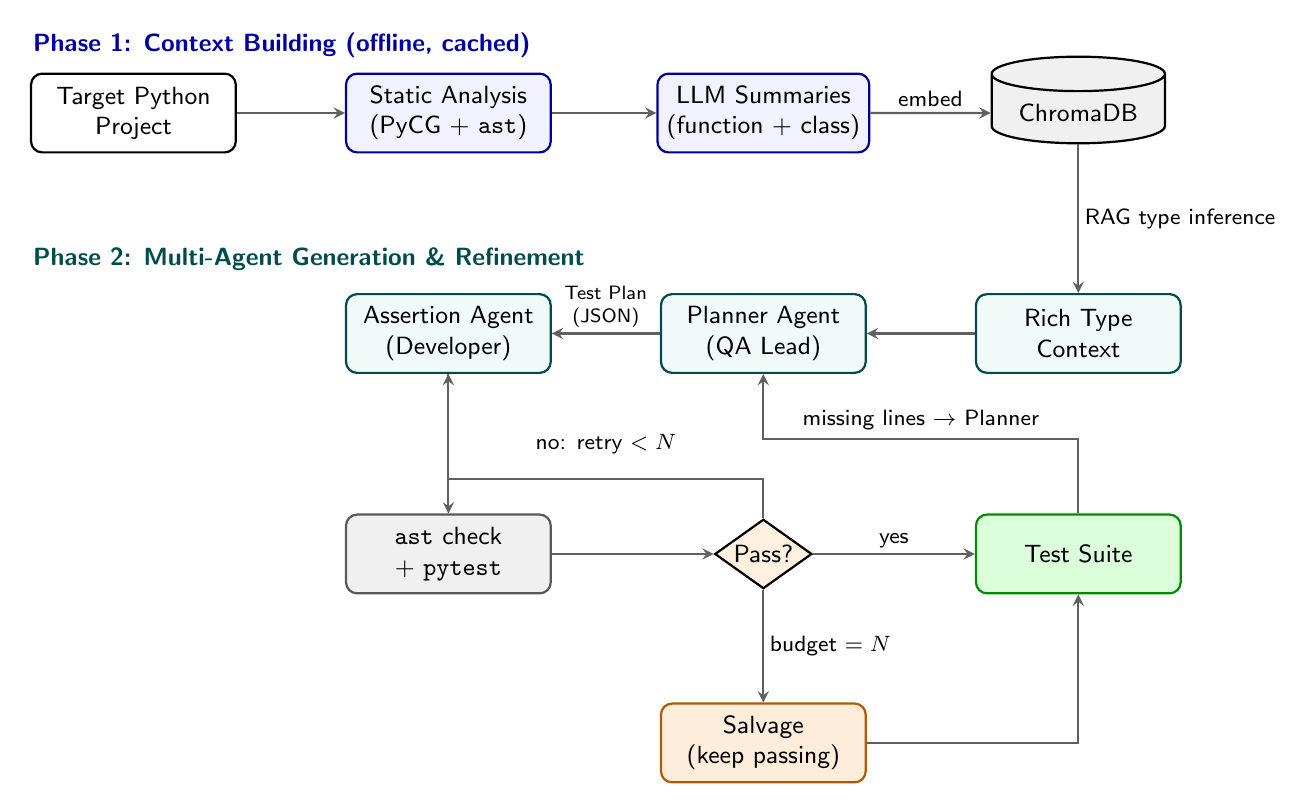
\begin{tikzpicture}[
      >=stealth,
      base/.style={draw, rounded corners, align=center, minimum height=1.0cm, minimum width=2.6cm, font=\sffamily\small, thick},
      p1/.style={base, fill=blue!5, draw=blue!60!black},
      p2/.style={base, fill=teal!5, draw=teal!60!black},
      io/.style={base, fill=white},
      store/.style={draw, cylinder, shape border rotate=90, aspect=0.25, align=center, fill=gray!12, minimum height=1.1cm, minimum width=2.2cm, font=\sffamily\small, thick},
      dec/.style={draw, diamond, aspect=1.4, align=center, fill=orange!12, font=\sffamily\small, thick, inner sep=1pt},
      done/.style={base, fill=green!14, draw=green!55!black},
      salv/.style={base, fill=orange!14, draw=orange!70!black},
      a/.style={->, thick, draw=gray!75!black},
      lbl/.style={font=\sffamily\footnotesize, inner sep=2pt}
    ]

    % ---- Linha 1: Phase 1, esquerda -> direita ----
    % Grelha alargada: posicoes x mudam de (0, 3.6, 7.2, 10.8) para (0, 4.0, 8.0, 12.0)
    \node[io]    (proj)   at (0,0)    {Target Python\\Project};
    \node[p1]    (static) at (4.0,0)  {Static Analysis\\(PyCG + \texttt{ast})};
    \node[p1]    (summ)   at (8.0,0)  {LLM Summaries\\(function + class)};
    \node[store] (chroma) at (12.0,0) {ChromaDB};

    \draw[a] (proj) -- (static);
    \draw[a] (static) -- (summ);
    \draw[a] (summ) -- node[lbl,above]{embed} (chroma);

    % ---- Linha 2: planeamento, direita -> esquerda ----
    \node[p2] (ctx)     at (12.0,-2.8) {Rich Type\\Context};
    \node[p2] (planner) at (8.0,-2.8)  {Planner Agent\\(QA Lead)};
    \node[p2] (dev)     at (4.0,-2.8)  {Assertion Agent\\(Developer)};

    \draw[a] (chroma) -- node[lbl,right]{RAG type inference} (ctx);
    \draw[a] (ctx) -- (planner);
    % O texto tem agora espaco de sobra entre as duas caixas
    \draw[a] (planner) -- node[lbl, above, align=center, font=\sffamily\scriptsize]{Test Plan\\(JSON)} (dev);

    % ---- Linha 3: validacao e retencao, esquerda -> direita ----
    \node[base, fill=gray!12, draw=gray!70!black] (val) at (4.0,-5.6) {\texttt{ast} check\\+ \texttt{pytest}};
    \node[dec]  (check) at (8.0,-5.6)  {Pass?};
    \node[done] (suite) at (12.0,-5.6) {Test Suite};
    \node[salv] (salv)  at (8.0,-8.0)  {Salvage\\(keep passing)};

    \draw[a] (dev) -- (val);
    \draw[a] (val) -- (check);
    \draw[a] (check) -- node[lbl,above]{yes} (suite);
    \draw[a] (check) -- node[lbl,right]{budget $=N$} (salv);
    \draw[a] (salv.east) -| (suite.south);

    % ---- Inner ReAct loop: check -> Assertion Agent ----
    \draw[a] (check.north) -- ++(0,0.5) -| (dev.south);
    % Ponto central da label ajustado de 5.4 para 6.0
    \node[lbl] at (6.0,-4.2) {no: retry $<N$};

    % ---- Outer coverage loop: suite -> Planner ----
    \draw[a] (suite.north) -- ++(0,0.95) -| (planner.south);
    % Ponto central da label ajustado de 9.0 para 10.0
    \node[lbl] at (10.0,-3.9) {missing lines $\rightarrow$ Planner};

    % ---- Rotulos de fase ----
    \node[lbl, anchor=south west, color=blue!65!black, font=\bfseries\sffamily\small]
      at (-1.35,0.62) {Phase 1: Context Building (offline, cached)};
    \node[lbl, anchor=south west, color=teal!60!black, font=\bfseries\sffamily\small]
      at (-1.35,-2.08) {Phase 2: Multi-Agent Generation \& Refinement};

    \end{tikzpicture}
    }
    \caption{Overview of the MARTA architecture.}
    \label{fig:architecture}
\end{figure}

The pipeline begins by constructing a \textit{Rich Type Context} (RTC) for the target function (Phase 1). Following TEST4PY~\cite{test4py2025}, MARTA combines structural program analysis with Retrieval-Augmented Generation (RAG). A global call graph is extracted using \texttt{PyCG}~\cite{salis2021pycg}, while Python's built-in \texttt{ast} parser is used to identify function signatures, class members, and dependency relationships. To complement this structural view, a LLM generates semantic descriptions of the codebase. For each function, the model produces both an implementation-oriented summary describing its behaviour and a requirement-oriented summary describing its intended purpose within the project. These are merged into a canonical \textit{Function Summary}, which is subsequently aggregated with structural information to form \textit{Class Summaries}. The resulting summaries are embedded and indexed within a vector database (\texttt{ChromaDB}~\cite{chromadb}), enabling retrieval of semantically related project components during generation.

When a target function is selected, MARTA infers candidate parameter types by analysing the methods and attributes accessed through each parameter. Project classes exposing compatible interfaces are identified and ranked according to their semantic similarity to the inferred behavioural role of the parameter. The resulting RTC combines the target source code, retrieved contextual information, inferred object types, and representative usage patterns required to instantiate and exercise the function under test.

Test generation is performed through two specialised agents (Phase 2). The \textit{Planner Agent} assumes the role of a Quality Assurance (QA) Lead and receives the RTC as input. Rather than generating executable code, the planner analyses the target behaviour and produces a structured test plan consisting of testing scenarios expressed in terms of preconditions, actions, and expected outcomes. During coverage-expansion rounds, the planner additionally receives a \texttt{COVERAGE FEEDBACK} field containing the lines and branches that remain uncovered. The planner is therefore responsible for deciding \textit{what} should be tested, while remaining completely agnostic to implementation details.

The generated plan acts as an explicit intermediate artifact and is passed to an \textit{Assertion Agent}, which assumes the role of a Software Developer. The Assertion Agent is responsible for translating the abstract scenarios into executable \texttt{Pytest} code~\cite{pytest}. Rather than generating one test case per request, it produces a complete test file containing all planned scenarios in a single inference step. This design provides whole-file context, allowing imports, fixtures, mocks, and shared dependencies to be declared once and reused consistently across the generated suite. Since behavioural reasoning has already been performed by the planner, the Assertion Agent focuses exclusively on implementation concerns such as object construction, dependency initialization, mock configuration, and assertion synthesis.


Generated test files are subsequently validated through an execution-driven refinement process. MARTA first uses Python's Abstract Syntax Tree (AST) parser to verify that the generated file is syntactically valid. Successfully parsed files are then executed against the code under test, allowing semantic and behavioural failures to be captured through runtime traces. When failures occur, MARTA enters an inner ReAct-style refinement loop in which exception messages, assertion failures, and runtime diagnostics are returned to the Assertion Agent together with the original test plan. The agent uses this information to iteratively repair the generated file while preserving the intended testing objective. This process continues until all tests pass or a predefined repair budget is exhausted.

Unlike existing approaches that repair or discard individual test cases, MARTA treats the complete test file as the unit of refinement. Consequently, when the repair budget is exhausted, the framework applies a \textit{salvage} strategy. Passing tests are identified from the execution report and only irreparable test functions are removed, while shared imports, fixtures, and supporting code are preserved. The resulting file is re-executed to ensure that all retained tests pass successfully. This mechanism prevents a single failing scenario from invalidating an otherwise useful suite and allows coverage accumulated during previous iterations to be preserved.

Finally, MARTA incorporates a second feedback loop dedicated to coverage expansion. After each refinement cycle, line and branch coverage are collected using \texttt{coverage.py}. The uncovered regions are attributed to their corresponding functions and returned exclusively to the Planner Agent through the \texttt{COVERAGE FEEDBACK} field. The planner then generates entirely new scenarios targeting the missing behaviour, which are translated into executable tests by the Assertion Agent and subjected to the same validation, repair, and salvage process. Unlike approaches that repeatedly modify existing tests, MARTA expands coverage by generating new behavioural hypotheses while preserving previously validated suites.



\section{Experimental Setup}
\label{sec:exp}

\subsection{Experimental Subjects and Baselines}

We evaluate MARTA on the established Python ATG benchmark originally introduced in the Pynguin evaluation~\cite{lukasczyk2022pynguin} and subsequently adopted by CodaMosa~\cite{lemieux2023codamosa} and CoverUp~\cite{altmayer2025coverup}. The benchmark comprises 486 target modules from 27 open-source Python projects, ranging from small utility libraries (e.g., \texttt{codetiming}, \texttt{sty}) to large and structurally complex frameworks (e.g., \texttt{ansible}, \texttt{black}). Using this benchmark facilitates direct comparison with prior work and ensures consistency with the evaluation setting established in the literature. More recent benchmarks, e.g. SWT-Bench~\cite{muendler2024swtbench}, focus on issue reproduction and patch validation rather than automated test generation and coverage maximization, making them less suitable for the objectives of this study.

We compare MARTA against two representative baselines. The first is Pynguin~\cite{lukasczyk2022pynguin}, the state-of-the-art SBST framework for Python, representing generation without language models. The second is a single-prompt LLM baseline derived from the generation component of TEST4PY~\cite{test4py2025}. To isolate the effect of MARTA's architectural decomposition, both LLM-based pipelines use the same Phase~1 context construction process, the same underlying model, the same repair budget, and the same execution environment. Since TEST4PY's published results were obtained using GPT-4o on a different benchmark configuration, we re-execute its generation module under our experimental conditions rather than comparing against the originally reported figures.
For contextual comparison, we additionally report the results published for CodaMosa~\cite{lemieux2023codamosa} and CoverUp~\cite{altmayer2025coverup}. These systems are not treated as direct baselines because they rely on frontier proprietary models and execution capabilities that were not reproducible within our local evaluation environment.

\subsection{Experimental Configuration}

To assess whether the benefits of MARTA generalize across model capacities, we evaluate the framework using two code-oriented language models. The primary evaluation, covering all 27 projects, employs DeepSeek-Coder-V2-Lite (16B), a mixture-of-experts model that activates approximately 2.4B parameters per token. To investigate whether the observed improvements persist with a stronger reasoning model, we additionally evaluate MARTA using Qwen2.5-Coder-32B.
%
Because serving a dense 32B model locally incurred substantially higher computational costs, the 32B evaluation was restricted to a fixed subset of ten projects (31 modules). This subset was selected prior to observing any 32B results and includes projects favouring MARTA, the single-prompt baseline, and Pynguin under the 16B configuration, reducing selection bias. Consequently, we treat the 32B experiment as exploratory evidence regarding model scaling rather than as a second full benchmark evaluation.
%
Both models were served locally through Ollama using the \texttt{BAAI/bge-large-en-v1.5} sentence embedding model for retrieval. All experiments were executed on the Deucalion HPC cluster using a node equipped with a single NVIDIA A100 (40GB) GPU, 32 CPU cores, and 200GB of RAM.

To ensure a fair comparison, each system constructs its own Phase~1 context independently rather than reusing cached artifacts. MARTA was executed with the temperature recommended during development ($T=0.2$), while the single-prompt baseline was executed with its original configuration ($T=0.0$). These settings were preserved to avoid misrepresenting the behaviour of the baseline. Both LLM-based systems were allocated the same repair budget ($N=3$ generation attempts per test file), used equivalent semantic context construction, and operated under the same execution environment.

\subsection{Evaluation Metrics}
We evaluate the proposed architecture with respect to the three objectives previously introduces: executability, structural adequacy, and fault-detection capability.

Following CoverUp~\cite{altmayer2025coverup}, we combine line and branch coverage into a single \emph{line+branch coverage} metric, computed with \texttt{coverage.py}~\cite{coveragepy} as the ratio of covered lines and branches to all coverable ones. A branch is considered covered only when all possible outcomes are exercised. Using the same metric facilitates direct comparison with previously published results on this benchmark family.

To evaluate fault-detection capability, we report \emph{mutation score} using \texttt{mutmut}~\cite{mutmut}. Mutation testing introduces small artificial faults into the source code and measures the proportion detected by the generated test suite. Since high structural coverage does not necessarily imply strong fault-detection capability, mutation score provides a complementary assessment of test effectiveness.

Finally, we report \emph{generation yield}, defined as the proportion of generated test files that survive the complete validation process and are ultimately delivered. This metric quantifies the cost of obtaining executable and fully validated test suites. \emph{Generation yield} is reported only for MARTA, which records all rejected candidates during generation. The single-prompt baseline was not instrumented to preserve discarded outputs, preventing an equivalent measurement. Pynguin is not directly comparable under this metric because it emits only tests that successfully execute during search.



\section{Results and Discussion}
\label{sec:res}

We compare MARTA against the single-prompt baseline (Test4Py) and the search-based
generator (Pynguin) across the 27 projects (486 modules) of our corpus.  The results below report the full
pipeline with its outer coverage-driven loop enabled (three generation rounds).

\subsection{Test Suite Yield and Oracle Strength}
\label{sec:oracles}

A recurring claim in LLM-based test generation is that richer context yields more
executable tests. Our data show that at this model scale the decisive difference
between architectures lies not in the \emph{size} of the delivered suite but in
\emph{what those tests actually verify}. Both LLM-based pipelines converge on
suites of comparable size while the search-based generator produces far fewer
(Table~\ref{tab:oracles}). Throughout this section, parametrized tests are expanded
to their number of cases.

\begin{table}[H]
\centering
\caption{Oracle strength of the generated suites (16B model, 27 projects).}
\label{tab:oracles}
\begin{tabular}{lrrrr}
\toprule
Tool & Tests & Asrt/test & No assertion & Weak \\
\midrule
MARTA    & 11{,}255 & 1.85 & 0.8\%  & 13.1\% \\
Test4Py  & 11{,}235 & 1.96 & 7.1\%  & 17.0\% \\
Pynguin  &  4{,}100 & 2.84 & 38.3\% & 30.4\% \\
\bottomrule
\end{tabular}
\end{table}


Both baselines deliver a substantial share of tests that execute code without
checking anything, that is, containing neither an assertion nor a
\texttt{pytest.raises}, where MARTA delivers almost none. They arrive there by
different routes. The
single-prompt system, once its repair budget is exhausted, removes assertions from a
test until it executes cleanly, whereas the search-based generator produces many
cases whose purpose is to reach a code path, with regression assertions attached only
where its assertion generator can supply them. In both, the reported size overstates what is verified. MARTA discards unrepairable tests outright rather than
hollowing them out.


The same asymmetry appears in assertion quality. We classify an assertion as
\emph{structurally weak} when it cannot distinguish correct from incorrect behaviour:
it checks a constant, the type of a value rather than the value itself, or a property
of a mock rather than of the code under test. Comparisons against literal values are
not penalised, since these are valid oracles. Under this criterion MARTA again has the lowest
share. Fig.~\ref{fig:oracles-example} shows the tests the three systems generated for
one function, illustrating the difference in oracle form that Table~\ref{tab:oracles}
aggregates. Both LLM-driven pipelines exercise it with concrete inputs and assert the return value, whereas the search-based generator reaches it once and records only that some input raises. MARTA also covers the exception path and a malformed exponent, neither of which the baseline's cases reach.

\begin{figure}[b]
\centering
\begin{lstlisting}[basicstyle=\ttfamily\scriptsize, breaklines=true, frame=single, backgroundcolor=\color{gray!5}]
# ---- MARTA -----------------------------------------------------
def test_valid_numbers():
    assert is_number('123') == True
    assert is_number('123.45') == True
    assert is_number('-123.45e6') == True

def test_invalid_inputs():
    assert is_number('abc') == False
    assert is_number('123abc') == False
    assert is_number('12.34e56f') == False   # malformed exponent

def test_error_handling():
    with pytest.raises(TypeError):
        is_number(None)

# ---- Test4Py (single-prompt) -----------------------------------
def test_valid_positive_integer():
    assert is_number('42') == True

def test_valid_negative_decimal():
    assert is_number('-9.12') == True

def test_valid_scientific_notation():
    assert is_number('1e3') == True

def test_invalid_string():
    assert is_number('1 2 3') == False

# ---- Pynguin (search-based) ------------------------------------
def test_case_6():
    bool_0 = False
    with pytest.raises(module_1.InvalidInputError):
        module_0.is_number(bool_0)
# Pynguin emits one module-level suite; its remaining cases
# target other functions in the same module.
\end{lstlisting}
\caption{Tests generated for \texttt{string\_utils.validation.is\_number} by the three systems (16B model, excerpts).}
\label{fig:oracles-example}
\end{figure}


The guarantee that every delivered test executes and asserts is obtained by
discarding. Across the 27 projects MARTA generated 13{,}589 candidate test files and retained
4{,}774 of them, quarantining the remaining 8{,}815. \emph{Generation yield} is therefore
35.1\%, equivalently a discard rate of 64.9\%. The 4{,}774 retained files hold the
11{,}255 test functions counted above. Because the baseline was not instrumented to
record its discarded candidates, we report this as a property of MARTA rather than as
a comparison. A rate of this
magnitude should be read against the capacity of the underlying model, which both LLM
pipelines share: it reflects what a model of this size produces on project-level
Python as much as it reflects either architecture and we would expect it to fall
with a stronger model, which the growth in retained tests at 32B
(Section~\ref{sec:model-capacity}) is consistent with.

Recovery is likewise not free and MARTA depends on it more: 52.6\% of its retained
files reached a passing state only after the salvage stage, against 19.7\% of the
baseline's, which reaches that state by stripping assertions from failing tests
rather than removing the tests themselves. The two also reject at different points. MARTA
validates syntax with \texttt{ast.parse}, which raises only on \texttt{SyntaxError}
and defers semantic rejection to execution, whereas the baseline gates on
\texttt{pylint --errors-only}, which additionally rejects undefined names, import
errors and missing members before any test is run. Pre-execution acceptance rates are
therefore not comparable across the two systems and we do not report them: MARTA
admits more candidates and prunes them against execution, whereas the baseline
rejects earlier and, for what survives, weakens rather than discards.

Decoupling generation into two agents could be expected to multiply inference cost,
since it introduces a planning call the single-prompt architecture does not make.
Measured end to end on a nine-project subset, MARTA costs 21\% more than the baseline
(13.4 against 11.1 GPU-hours), with the difference concentrated in context building
rather than in generation. Because the call graph, the generated summaries and the
vector index are persisted to disk under a content hash of the source, that step is
paid once per version of the code under test rather than on every run.

\subsection{Structural Coverage}
\label{sec:coverage}

The benchmark defines 486 \emph{modules} as its units of evaluation
\cite{lemieux2023codamosa} and we adopt that unit. The choice is consequential,
because the projects vary widely in size:
\texttt{codetiming} contributes a single module, whereas \texttt{ansible} alone
contributes 237, that is, 49\% of the benchmark, so averaging percentages over
projects would weight a one-module utility as heavily as a 237-module framework. We
therefore treat each module as one observation, taking the median and mean of the
per-module line+branch percentages, alongside a pooled measure as a weighting-free
confirmation. The pooled figure applies the same ratio once over the whole corpus
rather than per module, so it uses an identical denominator (68{,}248 coverable
elements) for the three tools and involves no weighting choice at all. Under every
aggregation, a module for which a tool produced no covering test counts as 0\% rather
than being excluded, so that a tool is not rewarded for declining to attempt the
hardest subjects. The per-module median additionally allows the search-based baseline
to be calibrated against published figures (Section~\ref{sec:calibration}). We note
that the single-prompt baseline's per-module median and pooled coverage coincide at
37.1\%. The two are computed independently and the agreement is a coincidence rather
than a transcription error.

\begin{table}[htpb]
\centering
\caption{\emph{line+branch coverage} over the 486 target modules (16B model).}
\label{tab:coverage}
\begin{tabular}{lrrr}
\toprule
Aggregation & MARTA & Test4Py & Pynguin \\
\midrule
\multicolumn{4}{l}{\textit{Per module (486 observations)}} \\
\quad Median            & 44.3\% & 37.1\% & 43.1\% \\
\quad Mean              & 45.2\% & 39.7\% & 44.8\% \\
\quad Pooled (overall)  & 40.6\% & 37.1\% & 35.3\% \\
\midrule
\multicolumn{4}{l}{\textit{Per project (27 observations)}} \\
\quad Mean              & 49.1\%          & 44.9\% & 54.7\% \\
\quad Median            & 42.1\%          & 43.3\% & 49.1\% \\
\bottomrule
\end{tabular}
\end{table}

At the module level (Table~\ref{tab:coverage}) MARTA ranks first on all three
measures and improves over the single-prompt baseline under every aggregation,
winning 19 of the 27 pairwise per-project comparisons. Averaged over projects,
however, Pynguin ranks first and the discrepancy between the two views is itself the
finding. Pynguin's advantage is concentrated in small, structurally simple modules
where evolutionary search can effectively exhaust the input space: it reaches 100\%
on \texttt{sty} (two modules) and 96.2\% on \texttt{codetiming} (one module). Such
projects are numerous but contribute few modules each, so they dominate a per-project
average while representing a small fraction of the benchmark. On the largest subjects
the ordering reverses: on \texttt{ansible} MARTA attains 40.0\% against Pynguin's
27.7\%, on \texttt{flutils} 66.6\% against 33.6\% and on \texttt{black} Pynguin
covers none of the target modules. This is precisely the coverage plateau that
motivated augmenting search with LLMs~\cite{lemieux2023codamosa}. We therefore read
the two views as complementary: search-based generation remains stronger and cheaper
for small, self-contained modules, while the multi-agent pipeline scales better to
the complex subjects that dominate the benchmark by module count.

One asymmetry in this comparison works against MARTA. An assertion-free test still
executes the code under test and therefore still earns coverage, so a suite carrying
many of them is structurally advantaged on this metric. MARTA leads at the module
level while carrying the fewest, by the margin reported in
Section~\ref{sec:oracles}.

\subsection{Fault-Revealing Capability}
\label{sec:mutation}

High coverage is a well-known vanity metric: executing a line does not imply
detecting a fault in it. Over the 27 projects (Table~\ref{tab:mutation}), MARTA
achieves a mean mutation score of 23.4\% against 20.9\% for the single-prompt
baseline and 17.2\% for Pynguin. It attains the highest score on 15 projects against
5 and 8 respectively. These counts sum to 28 rather than 27 because one project is tied and
counted for both tools involved. The comparison with Pynguin mirrors the divergence of
Section~\ref{sec:coverage}: it wins more per-project comparisons than the
single-prompt baseline (8 against 5) yet attains the lowest mean and median of the
three, for the same reason. This is consistent with the oracle rates of
Section~\ref{sec:oracles}: a suite in which most tests assert nothing accumulates
structural coverage without acquiring the ability to detect a regression.

The absolute values are low by the standards of full-suite mutation analysis and
deliberately so. Mutants are attributed to the module they belong to and evaluated
only against tests targeting that module, so a mutant killed incidentally by a test
written for another module counts as survived and modules for which a tool produced
no usable test contribute their mutants as survived rather than being excluded, so
that a tool is not rewarded for generating fewer tests. Both choices depress every
score uniformly, so the figures support the relative comparison under identical
attribution rather than comparison with full-suite scores reported elsewhere. One
asymmetry is worth noting: a generator optimising for minimal suites is disadvantaged
here, since fewer tests means fewer chances to kill a mutant, which is one reason the
search-based baseline sits below both LLM-based systems.


\begin{table}[htpb]
\centering
\caption{\emph{mutation score} under per-module attribution (16B model, 27 projects).}
\label{tab:mutation}
\begin{tabular}{lrrr}
\toprule
Tool & Mean & Median & Best on \\
\midrule
MARTA    & 23.4\% & 17.0\% & 15 projects \\
Test4Py  & 20.9\%          & 15.8\%          & 5 projects \\
Pynguin  & 17.2\%          & 11.4\%          & 8 projects \\
\bottomrule
\end{tabular}
\end{table}

\subsection{Calibration Against Published Results}
\label{sec:calibration}

Our conclusions rest on two baselines that we re-execute ourselves, so a
misconfigured baseline would inflate our results without any architectural merit.
The benchmark's shared lineage lets us check this directly for the search-based
baseline. CodaMosa~\cite{lemieux2023codamosa} is Pynguin augmented with an LLM and
reports a per-module median line+branch coverage of 47.0\% on this benchmark,
whereas our re-execution of Pynguin alone yields 43.1\%. The residual gap of roughly
four percentage points is consistent with the contribution attributed to the LLM
component in the original work, indicating that our search-based baseline is
configured in line with the published setup rather than inadvertently handicapped.

For external reference, the strongest published result on this benchmark family is
CoverUp~\cite{altmayer2025coverup}: on the 425 target modules our evaluations share,
its released report gives a per-module median of 79.6\% and pooled coverage of
60.3\%, against 42.8\% and 40.2\% for MARTA. We could not re-execute it, as it
depends on tool-calling behaviour our locally served models did not support, so this
is not a controlled comparison. CoverUp is driven by GPT-4o and every system we
execute by a locally served open-weights model, which leaves the model as the
principal difference and makes this a reference point for what the benchmark supports
under a frontier model rather than a comparison of architectures.
Section~\ref{sec:model-capacity} varies only the model, which is the controlled
version of the same question.


\subsection{Effect of Model Capacity}
\label{sec:model-capacity}

Every result reported so far holds the model fixed at 16B. To probe whether the architectural advantage persists as capacity grows, we evaluate MARTA and the single-prompt baseline on the ten-project subset (31 modules) using Qwen2.5-Coder-32B.

Any LLM-based tool is expected to improve with a stronger model. The critical finding
is how the \textit{relative} gains are distributed. As
Table~\ref{tab:capacity} shows, MARTA benefits more from the increased capacity than
the single-prompt baseline: the mean coverage gap between the two architectures widens
from 3.1 to 10.2 percentage points and the mutation score advantage grows from 1.6 to
5.6 points. If the multi-agent decoupling merely compensated for a weak 16B model,
this gap would shrink at 32B. Instead, MARTA leverages the stronger model more
effectively, indicating that separating planning from syntax scales at least as well
as an overloaded single prompt rather than being a workaround for limited capacity.
The subset is small, so this supports the direction of the effect more than its
magnitude.

\begin{table}[htbp]
\centering
\caption{Effect of model capacity on the ten-project subset (31 modules).}
\label{tab:capacity}
\begin{tabular}{lrr}
\toprule
Measure & 16B & 32B \\
\midrule
\emph{line+branch coverage} (pooled) & 56.0\% & 77.2\% \\
\emph{mutation score}                & 31.5\% & 54.0\% \\
Retained tests                & 777    & 1{,}676 \\
Tests with no assertion       & 0.2\%  & 0.2\% \\
Weak assertions               & 11.8\% & 4.8\% \\
\midrule
\multicolumn{3}{l}{\textit{Mean gap to single-prompt baseline (pp)}} \\
\quad \emph{line+branch} coverage    & $+$3.1 & $+$10.2 \\
\quad \emph{mutation score}          & $+$1.6 & $+$5.6 \\
\bottomrule
\end{tabular}
\end{table}

The comparison with the search-based baseline carries the same caveat but is more
striking. At 16B, the ordering on these ten projects reflects the
small-module regime where search excels (Section~\ref{sec:coverage}): Pynguin
(65.4\%) $>$ MARTA (56.0\%) $>$ Test4Py (52.8\%). Because Pynguin uses no language
model, its performance is static across this comparison. At 32B, MARTA reaches 77.2\%
coverage and overturns that lead, suggesting that with enough model capacity the
decoupled architecture can cross the search-based plateau even where evolutionary
search is strongest.



Finally, the oracle measurements separate the architectural contribution from raw
model capability. The share of assertion-free tests remains static at 0.2\% across
both models, as this is dictated by MARTA's retention policy.
The share of \textit{weak} assertions, by contrast, falls by more than half, from
11.8\% to 4.8\%, because writing an assertion that discriminates behaviour depends on
how well the model understands the target function. The two rates therefore move
independently: the model sets how good an assertion is, the architecture whether a
test without one is kept.


\section{Threats to Validity}
\label{sec:val}

\subsection{Internal Validity}
\label{sec:internal-validity}

To attribute the observed improvements to the generation architecture rather than to
the surrounding conditions, we held the semantic context, the underlying LLM, the
repair budget ($N=3$) and the execution environment constant across MARTA and the
single-prompt baseline. The one parameter that differs is the decoding temperature,
where we preserved the authors' original values to avoid misrepresenting the
published baseline. Due to the computational cost of local inference, each
configuration was executed once, so we cannot separate architectural effects from
run-to-run sampling variance. We mitigate this by reporting central tendencies over a
large number of paired observations rather than aggregate totals and per-project win
counts alongside means, so that a single outlying project cannot drive a reported
difference. All metrics are computed through a uniform, isolated measurement pipeline
applied equally to all tools and prompt-engineering bias is mitigated by reusing the
baseline's original TEST4PY~\cite{test4py2025} generation prompt unchanged. LLM
memorization of public repositories cannot be excluded, but would affect both systems
equally.

MARTA differs from the baseline in the generation architecture
as a whole, not in one isolated parameter and its mechanisms are not independent:
file-level generation and per-test salvage are possible because an explicit plan
exists and that plan exists because planning was separated from syntax. An ablation
removing the decomposition while retaining its consequences is therefore not well
defined. What the design does establish is that the semantic context, the model, the
repair budget and the execution environment are equivalent across the two systems, so
the measured differences are properties of the architecture rather than of the
information available to it.

\subsection{External Validity}
The benchmark subjects are predominantly small-to-medium open-source utilities, so
results may differ for large industrial codebases or projects relying heavily on
C-extensions or external I/O. Our two open-weights models indicate a direction with
respect to model capacity but do not establish a scaling law and the magnitude of
the decoupling benefit may differ for other model families or frontier API models.
The context-building and validation stages are specific
to the Python toolchain (\texttt{PyCG}, \texttt{ast}, \texttt{Pytest},
\texttt{coverage.py}) and transferring MARTA to another dynamically typed language
would require re-implementing that layer.

\subsection{Construct Validity}

Coverage alone does not fully capture test effectiveness. To mitigate this threat, we complement structural coverage with mutation score and \emph{generation-yield} measurements. Mutation scores are computed under per-module attribution rather than full-suite evaluation and therefore should not be compared directly with mutation-testing studies using global test suites. Similarly, the reported weak-assertion rates provide a conservative estimate of oracle quality rather than an exhaustive characterisation of assertion strength. Finally, because generated regression tests encode the current behaviour of the system under test, they evaluate the ability of a suite to detect future behavioural deviations rather than defects already present at generation time.



\section{Conclusion}
\label{sec:conc}

This paper presented MARTA, a Python regression test generation pipeline that separates abstract test planning from concrete test implementation. By introducing test plans as explicit intermediate artifacts, MARTA enables file-level generation, execution-driven repair, and coverage-guided refinement within a unified workflow. The resulting architecture allows behavioural reasoning and code synthesis to be addressed independently, reducing the burden placed on a single LLM generation step.
%
The empirical evaluation on a benchmark comprising 27 open-source Python projects (486 modules) shows that MARTA consistently outperforms both a search-based generator and a single-prompt LLM baseline. In addition to achieving the highest structural coverage and mutation scores, MARTA substantially reduces the number of assertion-free tests, indicating that the benefits of decomposition extend beyond executability and coverage to the verification quality of the generated suites. The observed advantage persists across different model capacities, suggesting that the improvements arise from the generation architecture itself rather than from a particular language model.

Future work will explore the use of the Planner Agent for security-oriented test generation, including adversarial inputs and robustness-focused scenarios. We also plan to investigate the integration of MARTA into CI/CD workflows and evaluate its behaviour with frontier language models and larger industrial codebases.

The artifact accompanying this paper, including the source code, evaluation scripts, and generated test suites, is available for anonymous review at \url{https://anonymous.4open.science/r/MARTA-3EFE/}. Additional material omitted for space, including generation traces, repair examples, and inference-cost analyses, is also provided. The artifact will be publicly archived with a DOI in the camera-ready version.

\bibliographystyle{splncs04}
\bibliography{references}

\end{document}